\documentclass[border=4pt]{standalone}
\usepackage{tikz}
\usetikzlibrary{arrows.meta,positioning,calc,fit,backgrounds,patterns,shapes.geometric}
\usepackage{amsmath,amssymb}
\usepackage{mathptmx}
\definecolor{lost}{HTML}{C2362D}
\definecolor{kept}{HTML}{17875A}
\definecolor{evid}{HTML}{3056D3}
\definecolor{ink}{HTML}{1D1D1F}
\definecolor{muted}{HTML}{6E6E73}
\tikzset{
  box/.style={draw=ink!70, rounded corners=2pt, align=center, fill=white, inner sep=4pt, font=\footnotesize},
  arr/.style={-{Stealth[length=2mm]}, draw=ink!70, line width=0.6pt},
  grp/.style={draw=muted!60, dashed, rounded corners=4pt, inner sep=7pt},
  lossbox/.style={draw=lost!80, fill=lost!6, text=lost!85!black, rounded corners=2pt, align=left, font=\footnotesize, inner sep=4pt},
  fixbox/.style={draw=kept!80, fill=kept!7, text=kept!65!black, rounded corners=2pt, align=left, font=\footnotesize, inner sep=4pt},
  dec/.style={diamond, aspect=2.2, draw=ink!70, fill=evid!6, align=center, font=\footnotesize, inner sep=1.5pt},
  lbl/.style={font=\footnotesize\bfseries, text=ink},
}

\begin{document}
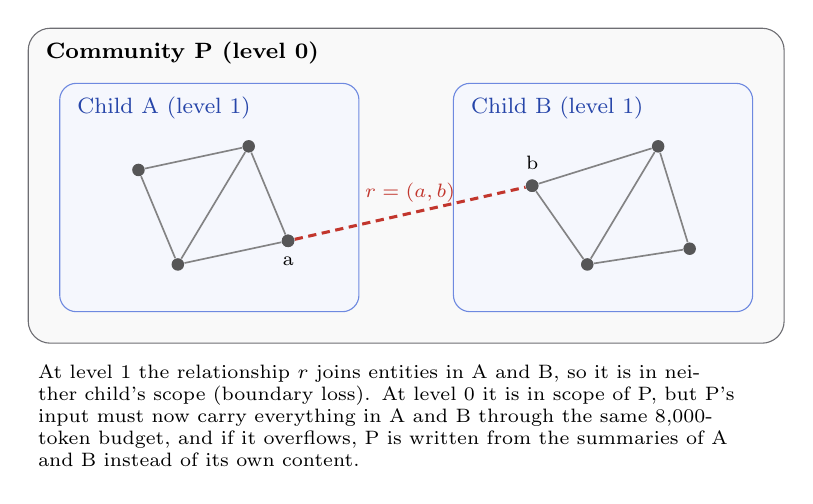
\begin{tikzpicture}[v/.style={circle, fill=ink!75, inner sep=1.6pt}, e/.style={draw=ink!55, line width=0.6pt}]
% level 0 community P with two children A and B
\draw[draw=muted, rounded corners=8pt, fill=muted!4] (-0.4,-0.4) rectangle (9.2,3.6);
\node[font=\footnotesize\bfseries, anchor=north west] at (-0.3,3.55) {Community P (level 0)};
\draw[draw=evid!70, rounded corners=6pt, fill=evid!5] (0,0) rectangle (3.8,2.9);
\node[font=\footnotesize, anchor=north west, text=evid!80!black] at (0.1,2.85) {Child A (level 1)};
\draw[draw=evid!70, rounded corners=6pt, fill=evid!5] (5.0,0) rectangle (8.8,2.9);
\node[font=\footnotesize, anchor=north west, text=evid!80!black] at (5.1,2.85) {Child B (level 1)};
\node[v] (a) at (1.0,1.8) {}; \node[v] (a2) at (2.4,2.1) {}; \node[v] (a3) at (1.5,0.6) {}; \node[v, label={[font=\scriptsize]below:a}] (a4) at (2.9,0.9) {};
\node[v, label={[font=\scriptsize]above:b}] (b) at (6.0,1.6) {}; \node[v] (b2) at (7.6,2.1) {}; \node[v] (b3) at (6.7,0.6) {}; \node[v] (b4) at (8.0,0.8) {};
\draw[e] (a)--(a2) (a)--(a3) (a2)--(a4) (a3)--(a4) (a2)--(a3);
\draw[e] (b)--(b2) (b)--(b3) (b2)--(b4) (b3)--(b4) (b2)--(b3);
\draw[draw=lost, line width=1.1pt, dash pattern=on 3pt off 2pt] (a4) -- node[above, font=\scriptsize, text=lost, pos=0.5] {$r=(a,b)$} (b);
\node[v] at (a4) {}; \node[v] at (b) {};
\node[font=\scriptsize, align=left, text width=8.9cm, anchor=north west] at (-0.4,-0.55) {At level 1 the relationship $r$ joins entities in A and B, so it is in neither child's scope (boundary loss). At level 0 it is in scope of P, but P's input must now carry everything in A and B through the same 8,000-token budget, and if it overflows, P is written from the summaries of A and B instead of its own content.};
\end{tikzpicture}
\end{document}
